\section{Extracting Structure} \label{sec:hrep}

In this section we present a compositional representation to express the random
generation of values following the internal structure of their data types along
with the structure present on patterns matchings and abstract interfaces.


The key idea of this work is to represent different sources of structured value
information of a data type in a homogeneous way that we call a ``higher-level
representation'' (|HRep| from now on).%
\footnote{The notion of higher-level comes from that the generation process of
  given target data type is entirely determined by the type of the chosen type
  level representation, instead of by a concrete generator defined at the term
  level.}
%
For this purpose, we use a series of automatically derived data types, each one
representing an atomic unit of information that can be randomly generated and
then reflected back to the corresponding value of the original data type.
%
Later, the user can compose these atomic representations using the provided type
level combinators in different ways into a ``generation specification'' that
completely determines the generation process.


We wil reuse the previously defined data type |Exp| and the function |foo| to
explain the different concepts involved all across this section.


\subsection*{\textbf{Representing Data Constructors}}

We begin by introducing the simplest data type representation that we can
extract from our codebase: the representation of single data constructor.
%
Each data constructor can be represented by an automatically derived data type
consisting of a single constructor with the same fields as the original, except
for the recursive ones that are abstracted away.
%
In this light, we represent each constructor of the data type |Exp| as follows:

\begin{code}
data HRep_Val  r = Mk_Val Int
data HRep_Add  r = Mk_Add r r
data HRep_Mul  r = Mk_Mul r r
\end{code}

Note that the previous definitions are type parametric over the type parameter
|r|.
%
This allow us to replace |r| with any concrete data type, obtaining different
possible values on each case.
%
For instance, the value (|Mk_Add 10 20|) has type |HRep_Add Int|, while the
value (|Mk_Mul True False|) has type |HRep_Mul Bool|.
%
In practice, this parametricity let us instatiate |r| with the type of the
chosen generation specification (which might be composed of several |HRep|s),
without having to modify anything in the underlying machinery.


Having the |HRep| of each data constructor, we can define an evaluation relation
($\evalrep{\_}{t} : |HRep|_f \rightarrow t$) that maps a value from each
representation |f| back to the target data type |t|.
%
Then, we simply need to translate each constructor representation back into its
corresponding one, translating the abstracted fields recursively:
%
\begin{alignat*}{4}
  &\evalrep{|Mk_Val|\ n\ \ \ &&}{|Exp|}
    &&= |Val|\ n \\
  &\evalrep{|Mk_Add|\ x\ y   &&}{|Exp|}
    &&= |Add|\ \evalrep{x}{Exp}\ \evalrep{y}{Exp} \\
  &\evalrep{|Mk_Mul|\ x\ y   &&}{|Exp|}
    &&= |Mul|\ \evalrep{x}{Exp}\ \evalrep{y}{Exp}
\end{alignat*}

The last missing piece is to automatically derive a random generators for each
constructor |HRep|.
%
For this purpose, it is important to consider that each constructor |HRep| has
its recursive fields abstracted away with a type parameter that will be later
instantiated with the generation specification type.
%
Given that this specification is unknown at the derivation time, we parametrize
each |HRep| generator with a random generator |gen_r| that is used to generate
each recursive fields:

\begin{code}
  gen_Val  gen_r  = Mk_Val  <$> arbitrary
  gen_Add  gen_r  = Mk_Add  <$> smaller gen_r <*> smaller gen_r
  gen_Mul  gen_r  = Mk_Mul  <$> smaller gen_r <*> smaller gen_r
\end{code} %$


\subsection*{\textbf{Type Level Combinators}}

In this work we define type level combinators which let the user combine the
automatically derived |HRep|s in several ways.
%
In first place, we define a type combinator (|term|) to tag a |HRep| to be
terminal, i.e., a representation that is allowed be generated when the
generation size gets exausted:
%
\begin{code}
data (f_term) a = Term (f a)
\end{code}

Additionally, we define a combinator ($\otimes$) to tag a |HRep| with an
explicit generation frequency $n$:

\begin{code}
data (f otimes n) a = Freq (f a)
\end{code}

The previous combinators only include information relevant to the generation
process, in a sense that neither one adds new structure to the final
representation.
%
In this light, they do not alter the evaluation semantics, and we translate them
back to our target data type by evaluating the inner representation:
%
\begin{alignat*}{4}
  &\evalrep{Freq\ x &&: f \otimes n &&}{t} &&= \evalrep{x : f}{t} \\
  &\evalrep{Term\ x &&: |f_term|    &&}{t} &&= \evalrep{x : f}{t}
\end{alignat*}

In the previous equations we explicitly annotate (using a colon) the type of the
evaluated term for clarity.
%
Later, to generate these combinators is enough to wrap a generated value from
the inner representation with the apropriate tag:

\begin{code}
gen_f_term     gen_r  = Term  <$> gen_f gen_r
gen_f_times_n  gen_r  = Freq  <$> gen_f gen_r
\end{code}


Perhaps more interesting, we define a combinator $(\oplus)$ to compose two
|HRep|s into a single one using a sum type to represent a random choice between
them:

\begin{code}
data (f oplus g) a = L (f a) | R (g a)
\end{code}

A composite representation built using $(\oplus)$ is transformed back into the
target data type by pattern matching on the data type variant and evaluating the
inner |HRep| accodingly:
%
\begin{alignat*}{3}
  &\evalrep{L\ x &&: f \oplus g}{t} = \evalrep{x : f &&}{t} \\
  &\evalrep{R\ x &&: f \oplus g}{t} = \evalrep{y : g &&}{t}
\end{alignat*}

Generating a composite |HRep| is slightly more complicated than before, as we
need to perform a random choice based on the generation size and the given
frequencies for each sub-represention:

\begin{code}
  gen_f_plus_g gen_r  = sized (\size ->
    if size == 0
    then frequency
      [ (freq0  at_f,  L  <$> gen_f  gen_r  )
      , (freq0  at_g,  R  <$> gen_g  gen_r  ) ]
    else frequency
      [ (freq at_f,  L  <$> gen_f  gen_r  )
      , (freq at_g,  R  <$> gen_g  gen_r  ) ])
\end{code} %$

In the previous definition, we reflect the type level frequencies of |f| and |g|
(|freq at_f| and |freq at_g|).
%
This reflection defaults to $1$ if the frequency tag ($\otimes$) is not present.
%
Then we use these frequencies to generate each inner |HRep| in the apropriate
proportion.
%
When the generation size gets exhausted, we reflect the terminal generation
frequency of each inner |HRep| in the same way as before (|freq0 at_f| and
|freq0 at_g|).
%
This time, however, we default the frequency reflection to $0$ for any inner
that not tagged as terminal, avoiding to generate non-terminal constructions in
the last step.


Later, we can use these combinators to create a type synonym |HRep_Exp| that
specifies a generation schema equivalent to the one seen in the concrete random
generator of type |Exp| presented in Section \ref{sec:randomtesting}:

\begin{code}
type HRep_Exp  =       HRep_Val_term
               oplus'  HRep_Add  otimes 2
               oplus'  HRep_Mul
\end{code}

However, a value of type |HRep_Exp| still has its recursive calls abstracted
away---the type parameter |r| is implicit at the definition of |HRep_Exp|.
%
We can think of it as a ``single layer'' of representation.
%
To make it able to represent recursive values we need to define a last type
level combinator to ``tie the knot'':

\begin{code}
  data Fix f = Fix (f (Fix f))
\end{code}

This datatype represents the \emph{fixed point} of a parametric data type |f|,
i.e., a data type where each recursive call gets instantiated with iself.
%
To translate fixed points back to our target data type we simply need translate
the inner representation:
%
\begin{align*}
  \evalrep{Fix\ x : Fix\ f}{t} = \evalrep{x : f}{t}
\end{align*}
%
Categorically, this generic transformation of fixed points is called a
\emph{catamorphism}, where our evaluation relation is known as its
\emph{algebra}.


Unlike the other combinators, to randomly generate a fixed point of a certain
representation |f|, we do not needt to parametrize the generation of the
recursive fields of the inner represention over an external generator |gen_r|.
%
Instead, we simply pipe the generation to the inner |HRep|, calling itself on
any recursive generation call that might appear inside:

\begin{code}
genFix_f = Fix <$> gen_f genFix_f
\end{code} %$

This way we obtain a concrete recursive generator for each representation |f|
that we define.
%
Then, we can define a random generator for our target data type simply by
generating a random value of our chosen representation, and transforming it back
to our target by the means of the evaluation relation:

\begin{code}
  gen_Exp = do  x <- genFix_HRep_Exp
                return eval_x_Exp
\end{code} %$


So far we have introduced the machinery required to represent the random
generation of a target data type considering only the structure encoded on its
definition.
%
However, this approach can now be easily extended to encode different sources of
structured information.
%
We proceed to introduce two extensions that help to address the problematic
testing scenarios presented in the previous section.


\subsection*{\textbf{Representing Pattern Matchings}}

We can follow a similar reasoning as before to represent the pattern matching
structure from a given function.
%
Consider the function |foo| defined in the previous section.
%
We can derive a new data type for each one of its pattern matchings, whose
fields represent each pattern variable present on the given pattern, abstracting
away every pattern variable of type |Exp|.
%
Concretely, we define the following data types:

\begin{code}
data HRep_foo_1  r = Mk_foo_1 r r
data HRep_foo_2  r = Mk_foo_2 Int r
\end{code}

The first pattern of |foo| contains two pattern variables (|x| and |y|) of type
|Exp| that are abstracted in the parametric fields of |Mk_foo_1|.
%
Similarly, the second pattern of |foo| contains the pattern variable |x| of type
|Int| represented by the first field of |Mk_foo_2|, along with the pattern
variable |y| of type |Exp| that also is abstracted in the second field of
|Mk_foo_2|.

To transform these representations back to our target data type, we simply
expand them it into the concrete value represented by the original pattern,
evaluating its fields back to |Exp| as well:
%
\begin{align*}
  &\evalrep{|Mk_foo_1|\ x\ y}{Exp} = \\
  &\ \ |Add (Add eval_x_Exp (Val 50)) (Add (Val 25) eval_y_Exp)|\\
  &\evalrep{|Mk_foo_2|\ x\ y}{Exp} = \\
  &\ \ |Mul (Val 50) (Mul (Val x) eval_y_Exp)|
\end{align*}

And the random generation of pattern |HRep|s is defined in the same way as we
did before for data constructors |HRep|s:

\begin{code}
  gen_foo_1  gen_r  = Mk_foo_1  <$> smaller gen_r  <*> smaller gen_r
  gen_foo_2  gen_r  = Mk_foo_2  <$> arbitrary      <*> smaller gen_r
\end{code} %$

Finally, we can join the pattern matching representation of each clause of |foo|
into a single one:

\begin{code}
type HRep_foo  = HRep_foo_1 oplus''  HRep_foo_2
\end{code}


\subsection*{\textbf{Representing Abstract Interfaces}}

To introduce the higher level representation of module abstract interfaces,
suppose we have a module |M| defining |Exp| combinators as follows:

\begin{code}
module M where

ten :: Exp
ten = Val 10

square :: Exp -> Exp
square x = Mul x x

minus :: Exp -> Exp -> Exp
minus x y = Add x (Mul y (Val (-1)))
\end{code}

We will represent each function of |M| returning a value of type |Exp| following
the same idea as before, deriving a data type with a single data constructor for
each one of them:

\begin{code}
data HRep_ten       r = Mk_ten
data HRep_square    r = Mk_square   r
data HRep_minus     r = Mk_minus    r r
\end{code}

In this case, each single constructor will have as fields the types of the
inputs of the function that they represent.
%
As before, we abstract away any field representing and input of type |Exp| with
a type parameter |r|.


To evaluate these representations, we simply pipe the values on its fields as
input parameter of each original function, returning its result.

\begin{alignat*}{3}
  &\evalrep{|Mk_ten|         &&}{Exp} = |ten| \\
  &\evalrep{|Mk_square|\ x   &&}{Exp} = |square eval_x_Exp| \\
  &\evalrep{|Mk_minus|\ x\ y &&}{Exp} = |minus  eval_x_Exp eval_y_Exp|
\end{alignat*}

Note that, by doing this, the generation process inherits any patology that the
functions we use to generate values might have.
%
For instance, if the function |square| is non-terminating for some inputs, our
generation process could suffer from this as well.
%
Furthermore, the generation procedure for abstract interface representations
follows the same pattern as before:

\begin{code}
  gen_ten     gen_r  = Mk_ten
  gen_square  gen_r  = Mk_square  <$> smaller gen_r
  gen_minus  gen_r   = Mk_minus   <$> smaller gen_r  <*> smaller gen_r
\end{code} %$

We will also define a type synonym to join all the representations of the module
|M| into a single one.

\begin{code}
type HRep_M  = HRep_ten oplus''  HRep_square oplus''  HRep_minus
\end{code}

Finally, we can put all the derived machinery together into a generation
specification |Exp_S|, assigning (possibly) different generation frequencies to
each individual |HRep| we combine:

\begin{code}
type Exp_S  =       HRep_Exp  otimes 4
            oplus'  HRep_foo  otimes 2
            oplus'  HRep_M
\end{code}

This previous definition can be interpreted graphically as it is shown in the
Figure \ref{fig:hrep}, where curly arrows represent the structural information
extracted using meta-programming.

\begin{figure}[t]
  \centering
  \section{Extracting Structure} \label{sec:hrep}

In this work, we ...

\begin{code}
data HRep_Val  a = Mk_Val Int
data HRep_Add  a = Mk_Add a a
data HRep_Mul  a = Mk_Mul a a
\end{code}

For this purpose, we employ Haskell's type classes mechanism \tocite{}.
%
We define an evaluation type class $(\Downarrow)$ which specifies how to perform
a single transformation |step| from the higher-order representation back into a
concrete value of the target:

\begin{code}
class (rep down target) where
  step :: rep target -> target
\end{code}

Then, we can define the following overloaded instances of the |step| operation
for the canonical representations of data constructors simply by mapping each
lifted constructor back into its corresponding one.

\begin{code}
instance (HRep_Val down Exp) where
  step (Mk_Val n) = Val n

instance (HRep_Add down Exp) where
  step (Mk_Add x y) = Add x y

instance (HRep_Mul down Exp) where
  step (Mk_Mul x y) = Mul x y
\end{code}

With these individual representations, we can define a type combinator
$(\oplus)$ to compose two representations into a single one:

\begin{code}
data (f oplus g) a = L (f a) | R (g a)
\end{code}

Then, a composite representation can be transformed back into the concrete
target type by pattern matching on the data type variant and applying the |step|
tranformation to the inner representation:

\begin{code}
instance (f oplus g down Exp) where
  step (L f) = step f
  step (R g) = step g
\end{code}

Furthermore, we can define a type combinator ($\otimes$) to tag every
representation with an explicit generation frequency:

\begin{code}
data (f otimes n) a = Freq (f a)
\end{code}

This combinator is evaluated back to our target data type simply by piping the
result from the inner representation.
%
It does not change the evaluation semantics, as it is only considered at
generation time:

\begin{code}
instance (f otimes n down Exp) where
  step (Freq f) = step f
\end{code}

With the introduced combinators, we can easily create a type synonym |HRep_Exp|
to refer to the canonical representation of our original data type |Exp|,
tagging for instance the representation of the constuctor |Add| to be generated
in double the proportion of rest of the representations:

\begin{code}
type HRep_Exp  =       HRep_Val
               oplus'  HRep_Add  otimes 2
               oplus'  HRep_Mul
\end{code}



\begin{code}
data HRep_foo_1  a = Mk_foo_1 a a
data HRep_foo_2  a = Mk_foo_2 Int a
\end{code}

\begin{code}
instance (HRep_foo_1 down Exp) where
  step (Mk_foo_1 x y)
    = Add (Add x (Val 50)) (Add (Val 25) y)

instance (HRep_foo_2 down Exp) where
  step (Mk_foo_2 x y)
    = Mul (Val 50) (Mul (Val x) y)
\end{code}

\begin{code}
type HRep_foo  =       HRep_foo_1
               oplus'  HRep_foo_2
\end{code}


\begin{code}
data HRep_ten       a = Mk_ten
data HRep_square    a = Mk_square   a
data HRep_minus     a = Mk_minus    a a
\end{code}

\begin{code}
instance (HRep_ten down Exp) where
  step Mk_ten = ten

instance (HRep_square down Exp) where
  step (Mk_square x) = square x

instance (HRep_minus down Exp) where
  step (Mk_minus x y) = minus x y
\end{code}


\begin{code}
type HRep_M  =       HRep_ten
             oplus'  HRep_square
             oplus'  HRep_minus
\end{code}



\begin{code}
type Spec_Exp  =       HRep_Exp  otimes 4
               oplus'  HRep_foo  otimes 2
               oplus'  HRep_M
\end{code}

This previous definition can be interpreted graphically as it is shown in the
Figure \ref{fig:hrep}.
%
Curly arrows represent the structural information extracted using
meta-programming.

\begin{figure}[t]
  \centering
  \section{Extracting Structure} \label{sec:hrep}

In this work, we ...

\begin{code}
data HRep_Val  a = Mk_Val Int
data HRep_Add  a = Mk_Add a a
data HRep_Mul  a = Mk_Mul a a
\end{code}

For this purpose, we employ Haskell's type classes mechanism \tocite{}.
%
We define an evaluation type class $(\Downarrow)$ which specifies how to perform
a single transformation |step| from the higher-order representation back into a
concrete value of the target:

\begin{code}
class (rep down target) where
  step :: rep target -> target
\end{code}

Then, we can define the following overloaded instances of the |step| operation
for the canonical representations of data constructors simply by mapping each
lifted constructor back into its corresponding one.

\begin{code}
instance (HRep_Val down Exp) where
  step (Mk_Val n) = Val n

instance (HRep_Add down Exp) where
  step (Mk_Add x y) = Add x y

instance (HRep_Mul down Exp) where
  step (Mk_Mul x y) = Mul x y
\end{code}

With these individual representations, we can define a type combinator
$(\oplus)$ to compose two representations into a single one:

\begin{code}
data (f oplus g) a = L (f a) | R (g a)
\end{code}

Then, a composite representation can be transformed back into the concrete
target type by pattern matching on the data type variant and applying the |step|
tranformation to the inner representation:

\begin{code}
instance (f oplus g down Exp) where
  step (L f) = step f
  step (R g) = step g
\end{code}

Furthermore, we can define a type combinator ($\otimes$) to tag every
representation with an explicit generation frequency:

\begin{code}
data (f otimes n) a = Freq (f a)
\end{code}

This combinator is evaluated back to our target data type simply by piping the
result from the inner representation.
%
It does not change the evaluation semantics, as it is only considered at
generation time:

\begin{code}
instance (f otimes n down Exp) where
  step (Freq f) = step f
\end{code}

With the introduced combinators, we can easily create a type synonym |HRep_Exp|
to refer to the canonical representation of our original data type |Exp|,
tagging for instance the representation of the constuctor |Add| to be generated
in double the proportion of rest of the representations:

\begin{code}
type HRep_Exp  =       HRep_Val
               oplus'  HRep_Add  otimes 2
               oplus'  HRep_Mul
\end{code}



\begin{code}
data HRep_foo_1  a = Mk_foo_1 a a
data HRep_foo_2  a = Mk_foo_2 Int a
\end{code}

\begin{code}
instance (HRep_foo_1 down Exp) where
  step (Mk_foo_1 x y)
    = Add (Add x (Val 50)) (Add (Val 25) y)

instance (HRep_foo_2 down Exp) where
  step (Mk_foo_2 x y)
    = Mul (Val 50) (Mul (Val x) y)
\end{code}

\begin{code}
type HRep_foo  =       HRep_foo_1
               oplus'  HRep_foo_2
\end{code}


\begin{code}
data HRep_ten       a = Mk_ten
data HRep_square    a = Mk_square   a
data HRep_minus     a = Mk_minus    a a
\end{code}

\begin{code}
instance (HRep_ten down Exp) where
  step Mk_ten = ten

instance (HRep_square down Exp) where
  step (Mk_square x) = square x

instance (HRep_minus down Exp) where
  step (Mk_minus x y) = minus x y
\end{code}


\begin{code}
type HRep_M  =       HRep_ten
             oplus'  HRep_square
             oplus'  HRep_minus
\end{code}



\begin{code}
type Spec_Exp  =       HRep_Exp  otimes 4
               oplus'  HRep_foo  otimes 2
               oplus'  HRep_M
\end{code}

This previous definition can be interpreted graphically as it is shown in the
Figure \ref{fig:hrep}.
%
Curly arrows represent the structural information extracted using
meta-programming.

\begin{figure}[t]
  \centering
  \section{Extracting Structure} \label{sec:hrep}

In this work, we ...

\begin{code}
data HRep_Val  a = Mk_Val Int
data HRep_Add  a = Mk_Add a a
data HRep_Mul  a = Mk_Mul a a
\end{code}

For this purpose, we employ Haskell's type classes mechanism \tocite{}.
%
We define an evaluation type class $(\Downarrow)$ which specifies how to perform
a single transformation |step| from the higher-order representation back into a
concrete value of the target:

\begin{code}
class (rep down target) where
  step :: rep target -> target
\end{code}

Then, we can define the following overloaded instances of the |step| operation
for the canonical representations of data constructors simply by mapping each
lifted constructor back into its corresponding one.

\begin{code}
instance (HRep_Val down Exp) where
  step (Mk_Val n) = Val n

instance (HRep_Add down Exp) where
  step (Mk_Add x y) = Add x y

instance (HRep_Mul down Exp) where
  step (Mk_Mul x y) = Mul x y
\end{code}

With these individual representations, we can define a type combinator
$(\oplus)$ to compose two representations into a single one:

\begin{code}
data (f oplus g) a = L (f a) | R (g a)
\end{code}

Then, a composite representation can be transformed back into the concrete
target type by pattern matching on the data type variant and applying the |step|
tranformation to the inner representation:

\begin{code}
instance (f oplus g down Exp) where
  step (L f) = step f
  step (R g) = step g
\end{code}

Furthermore, we can define a type combinator ($\otimes$) to tag every
representation with an explicit generation frequency:

\begin{code}
data (f otimes n) a = Freq (f a)
\end{code}

This combinator is evaluated back to our target data type simply by piping the
result from the inner representation.
%
It does not change the evaluation semantics, as it is only considered at
generation time:

\begin{code}
instance (f otimes n down Exp) where
  step (Freq f) = step f
\end{code}

With the introduced combinators, we can easily create a type synonym |HRep_Exp|
to refer to the canonical representation of our original data type |Exp|,
tagging for instance the representation of the constuctor |Add| to be generated
in double the proportion of rest of the representations:

\begin{code}
type HRep_Exp  =       HRep_Val
               oplus'  HRep_Add  otimes 2
               oplus'  HRep_Mul
\end{code}



\begin{code}
data HRep_foo_1  a = Mk_foo_1 a a
data HRep_foo_2  a = Mk_foo_2 Int a
\end{code}

\begin{code}
instance (HRep_foo_1 down Exp) where
  step (Mk_foo_1 x y)
    = Add (Add x (Val 50)) (Add (Val 25) y)

instance (HRep_foo_2 down Exp) where
  step (Mk_foo_2 x y)
    = Mul (Val 50) (Mul (Val x) y)
\end{code}

\begin{code}
type HRep_foo  =       HRep_foo_1
               oplus'  HRep_foo_2
\end{code}


\begin{code}
data HRep_ten       a = Mk_ten
data HRep_square    a = Mk_square   a
data HRep_minus     a = Mk_minus    a a
\end{code}

\begin{code}
instance (HRep_ten down Exp) where
  step Mk_ten = ten

instance (HRep_square down Exp) where
  step (Mk_square x) = square x

instance (HRep_minus down Exp) where
  step (Mk_minus x y) = minus x y
\end{code}


\begin{code}
type HRep_M  =       HRep_ten
             oplus'  HRep_square
             oplus'  HRep_minus
\end{code}



\begin{code}
type Spec_Exp  =       HRep_Exp  otimes 4
               oplus'  HRep_foo  otimes 2
               oplus'  HRep_M
\end{code}

This previous definition can be interpreted graphically as it is shown in the
Figure \ref{fig:hrep}.
%
Curly arrows represent the structural information extracted using
meta-programming.

\begin{figure}[t]
  \centering
  \input{tikz/hrep.tex}
  \caption{Higher order representation of the data type |Exp|, using structural
    information from the function |foo| and the abstract interface of the module
    |M|.}
  \label{fig:hrep}
\end{figure}

% \begin{code}
% data (Term f) a = TagTerm (f a)

% instance (Term f down Exp) where
%   step (TagTerm f) = step f
% \end{code}
  \caption{Higher order representation of the data type |Exp|, using structural
    information from the function |foo| and the abstract interface of the module
    |M|.}
  \label{fig:hrep}
\end{figure}

% \begin{code}
% data (Term f) a = TagTerm (f a)

% instance (Term f down Exp) where
%   step (TagTerm f) = step f
% \end{code}
  \caption{Higher order representation of the data type |Exp|, using structural
    information from the function |foo| and the abstract interface of the module
    |M|.}
  \label{fig:hrep}
\end{figure}

% \begin{code}
% data (Term f) a = TagTerm (f a)

% instance (Term f down Exp) where
%   step (TagTerm f) = step f
% \end{code}
  \caption{Higher level representation of the data type |Exp|, defined using
    structural information from the function |foo| and the abstract interface of
    the module |M|.}
  \label{fig:hrep}
\end{figure}


We want to remark that, for space reasons, we were only able to introduce the
representation of a rather simple target data type.
%
In practice, this reasoning can be extended to mutually recursive and parametric
types as well.


Overall, we believe that this approach has some advantages over the usual
type-driven derivation of random generators:
%
\begin{itemize}
\item \textbf{Composability:} we can combine different atomic representations
  using different structure information sources depending on what property or
  sub-system we need to verify using random values.
  %
\item \textbf{Extensibility:} the developer can derive representations for new
  sources of structure information and combine them with the existing ones
  simply by adding them to the exiting representation of the target data type.
  %
\item \textbf{Predictability:} using branching processes theory, it is possible
  to predict the average distribution of generated values in terms of number of
  constructors.
  %
  This prediction is completely modular, and can be obtained for any composite
  representation obtained using the automatically derived |HRep|s and the
  provided combinators.
\end{itemize}

\todo[inline]{Maybe we can show an example random value from the representation
  and its corresponding target value }



% \begin{align*}
%   \llbracket \_ \rrbracket_{target}\ :\ rep_{target}\ \rightarrow\ target
% \end{align*}
%
% \begin{code}
% class (rep down target) where
%   step :: rep target -> target
% \end{code}
%
% \begin{code}
% data (Term f) a = TagTerm (f a)

% \begin{code}
% instance (HRep_Val down Exp) where
%   step (Mk_Val n) = Val n

% instance (HRep_Add down Exp) where
%   step (Mk_Add x y) = Add x y

% instance (HRep_Mul down Exp) where
%   step (Mk_Mul x y) = Mul x y
% \end{code}

% \begin{code}
% instance (f otimes n down Exp) where
%   step (Freq f) = step f
% \end{code}

% \begin{code}
% instance Arbitrary1 (f otimes n) where
%   liftArbitrary gen_HRep = Tag <$> gen_HRep
% \end{code} %$

% instance (Term f down Exp) where
%   step (TagTerm f) = step f
% \end{code}

% \begin{code}
% instance (HRep_ten down Exp) where
%   step Mk_ten = ten

% instance (HRep_square down Exp) where
%   step (Mk_square x) = square x

% instance (HRep_minus down Exp) where
%   step (Mk_minus x y) = minus x y
% \end{code}

% \begin{code}
% instance Arbitrary1 HRep_ten where
%   liftArbitrary gen_HRep = pure Mk_ten

% instance Arbitrary1 HRep_square where
%   liftArbitrary gen_HRep = Mk_square <$> gen_HRep

% instance Arbitrary1 HRep_minus where
%   liftArbitrary gen_HRep
%     = Mk_minus <$> gen_HRep <*> gen_HRep
% \end{code} %$

% \begin{code}
% instance (HRep_foo_1 down Exp) where
%   step (Mk_foo_1 x y)
%     = Add (Add x (Val 50)) (Add (Val 25) y)

% instance (HRep_foo_2 down Exp) where
%   step (Mk_foo_2 x y)
%     = Mul (Val 50) (Mul (Val x) y)
% \end{code}

% \begin{code}
% instance Arbitrary1 HRep_foo_1 where
%   liftArbitrary gen_HRep
%     = Mk_foo_1 <$> gen_HRep <*> gen_HRep

% instance Arbitrary1 HRep_foo_2 where
%   liftArbitrary gen_HRep
%     = Mk_foo_2 <$> arbitrary <*> gen_HRep
% \end{code} %$

% \begin{code}
% instance (f oplus g down Exp) where
%   step (L f) = step f
%   step (R g) = step g
% \end{code}

% \begin{code}
% instance Arbitrary1 (f oplus g) where
%   liftArbitrary gen_HRep
%     = frequency
%       [ (freq at_f, L <$> gen_HRep)
%       , (freq at_g, R <$> gen_HRep) ]
% \end{code} %$

% \begin{figure}[b]
%   \centering
%   
\tikzset{every picture/.style={line width=0.75pt}} %set default line width to 0.75pt

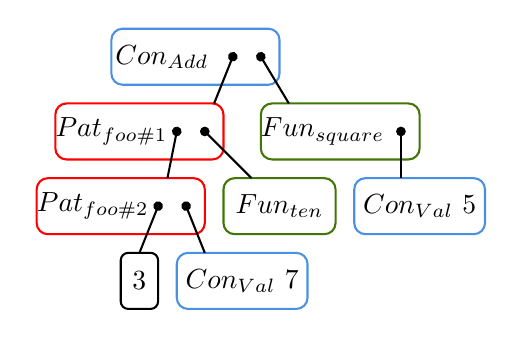
\begin{tikzpicture}[x=0.75pt,y=0.75pt,yscale=-0.9,xscale=0.9]
%uncomment if require: \path (0,440.8571319580078); %set diagram left start at 0, and has height of 440.8571319580078

%Rounded Rect [id:dp48618213158536694]
\draw  [color={rgb, 255:red, 74; green, 144; blue, 226 }  ,draw opacity=1 ] (190,196) .. controls (190,192.69) and (192.69,190) .. (196,190) -- (254,190) .. controls (257.31,190) and (260,192.69) .. (260,196) -- (260,214) .. controls (260,217.31) and (257.31,220) .. (254,220) -- (196,220) .. controls (192.69,220) and (190,217.31) .. (190,214) -- cycle ;

%Rounded Rect [id:dp009025103452140248]
\draw  [color={rgb, 255:red, 74; green, 144; blue, 226 }  ,draw opacity=1 ] (95,236) .. controls (95,232.69) and (97.69,230) .. (101,230) -- (159,230) .. controls (162.31,230) and (165,232.69) .. (165,236) -- (165,254) .. controls (165,257.31) and (162.31,260) .. (159,260) -- (101,260) .. controls (97.69,260) and (95,257.31) .. (95,254) -- cycle ;

%Rounded Rect [id:dp9232511876637792]
\draw  [color={rgb, 255:red, 74; green, 144; blue, 226 }  ,draw opacity=1 ] (60,116) .. controls (60,112.69) and (62.69,110) .. (66,110) -- (144,110) .. controls (147.31,110) and (150,112.69) .. (150,116) -- (150,134) .. controls (150,137.31) and (147.31,140) .. (144,140) -- (66,140) .. controls (62.69,140) and (60,137.31) .. (60,134) -- cycle ;

%Rounded Rect [id:dp10823094494105145]
\draw  [color={rgb, 255:red, 255; green, 0; blue, 0 }  ,draw opacity=1 ] (30,156) .. controls (30,152.69) and (32.69,150) .. (36,150) -- (114,150) .. controls (117.31,150) and (120,152.69) .. (120,156) -- (120,174) .. controls (120,177.31) and (117.31,180) .. (114,180) -- (36,180) .. controls (32.69,180) and (30,177.31) .. (30,174) -- cycle ;

%Rounded Rect [id:dp509725264431323]
\draw  [color={rgb, 255:red, 255; green, 0; blue, 0 }  ,draw opacity=1 ] (20,196) .. controls (20,192.69) and (22.69,190) .. (26,190) -- (104,190) .. controls (107.31,190) and (110,192.69) .. (110,196) -- (110,214) .. controls (110,217.31) and (107.31,220) .. (104,220) -- (26,220) .. controls (22.69,220) and (20,217.31) .. (20,214) -- cycle ;

%Rounded Rect [id:dp3455746100780601]
\draw   (65,234) .. controls (65,231.79) and (66.79,230) .. (69,230) -- (81,230) .. controls (83.21,230) and (85,231.79) .. (85,234) -- (85,256) .. controls (85,258.21) and (83.21,260) .. (81,260) -- (69,260) .. controls (66.79,260) and (65,258.21) .. (65,256) -- cycle ;

%Rounded Rect [id:dp5622973663481885]
\draw  [color={rgb, 255:red, 65; green, 117; blue, 5 }  ,draw opacity=1 ] (140,156) .. controls (140,152.69) and (142.69,150) .. (146,150) -- (219,150) .. controls (222.31,150) and (225,152.69) .. (225,156) -- (225,174) .. controls (225,177.31) and (222.31,180) .. (219,180) -- (146,180) .. controls (142.69,180) and (140,177.31) .. (140,174) -- cycle ;

%Rounded Rect [id:dp33414100410678915]
\draw  [color={rgb, 255:red, 65; green, 117; blue, 5 }  ,draw opacity=1 ] (120,196) .. controls (120,192.69) and (122.69,190) .. (126,190) -- (174,190) .. controls (177.31,190) and (180,192.69) .. (180,196) -- (180,214) .. controls (180,217.31) and (177.31,220) .. (174,220) -- (126,220) .. controls (122.69,220) and (120,217.31) .. (120,214) -- cycle ;

%Straight Lines [id:da7735002123972574]
\draw    (140,125) -- (155,150) ;

\draw [shift={(140,125)}, rotate = 59.04] [color={rgb, 255:red, 0; green, 0; blue, 0 }  ][fill={rgb, 255:red, 0; green, 0; blue, 0 }  ][line width=0.75]      (0, 0) circle [x radius= 2, y radius= 2]   ;
%Straight Lines [id:da19830589256441322]
\draw    (125,125) -- (115,150) ;

\draw [shift={(125,125)}, rotate = 111.8] [color={rgb, 255:red, 0; green, 0; blue, 0 }  ][fill={rgb, 255:red, 0; green, 0; blue, 0 }  ][line width=0.75]      (0, 0) circle [x radius= 2, y radius= 2]   ;
%Straight Lines [id:da7234273703208924]
\draw    (95,165) -- (90,190) ;

\draw [shift={(95,165)}, rotate = 101.31] [color={rgb, 255:red, 0; green, 0; blue, 0 }  ][fill={rgb, 255:red, 0; green, 0; blue, 0 }  ][line width=0.75]      (0, 0) circle [x radius= 2, y radius= 2]   ;
%Straight Lines [id:da39520289035501]
\draw    (110,165) -- (135,190) ;

\draw [shift={(110,165)}, rotate = 45] [color={rgb, 255:red, 0; green, 0; blue, 0 }  ][fill={rgb, 255:red, 0; green, 0; blue, 0 }  ][line width=0.75]      (0, 0) circle [x radius= 2, y radius= 2]   ;
%Straight Lines [id:da4431461097782077]
\draw    (215,165) -- (215,190) ;

\draw [shift={(215,165)}, rotate = 90] [color={rgb, 255:red, 0; green, 0; blue, 0 }  ][fill={rgb, 255:red, 0; green, 0; blue, 0 }  ][line width=0.75]      (0, 0) circle [x radius= 2, y radius= 2]   ;
%Straight Lines [id:da8121818084178258]
\draw    (85,205) -- (75,230) ;

\draw [shift={(85,205)}, rotate = 111.8] [color={rgb, 255:red, 0; green, 0; blue, 0 }  ][fill={rgb, 255:red, 0; green, 0; blue, 0 }  ][line width=0.75]      (0, 0) circle [x radius= 2, y radius= 2]   ;
%Straight Lines [id:da8679389234287274]
\draw    (100,205) -- (110,230) ;

\draw [shift={(100,205)}, rotate = 68.2] [color={rgb, 255:red, 0; green, 0; blue, 0 }  ][fill={rgb, 255:red, 0; green, 0; blue, 0 }  ][line width=0.75]      (0, 0) circle [x radius= 2, y radius= 2]   ;

% Text Node
\draw (225,205) node   {$Con_{Val} \ 5$};
% Text Node
\draw (130,245) node   {$Con_{Val} \ 7$};
% Text Node
\draw (87,125) node   {$Con_{Add}$};
% Text Node
\draw (60,165) node   {$Pat_{foo\#1}$};
% Text Node
\draw (50,205) node   {$Pat_{foo\#2}$};
% Text Node
\draw (75,245) node   {$3$};
% Text Node
\draw (173.05,165) node   {$Fun_{square}$};
% Text Node
\draw (150,205) node   {$Fun_{ten}$};

\end{tikzpicture}

%   \caption{Higher level representation of the data type |Exp|, defined using
%     structural information from the function |foo| and the abstract interface of
%     the module |M|.}
%   \label{fig:hrep}
% \end{figure}